\documentclass[UTF8,11pt]{ctexart}

% ======================
% 基础宏包
% ======================
\usepackage[a4paper,margin=2.4cm]{geometry}
\usepackage{setspace}
\usepackage{fancyhdr}
\usepackage{titlesec}
\usepackage{enumitem}
\setlist{itemsep=0.2em, parsep=0pt, topsep=0.3em}
\usepackage{multicol}
\usepackage{booktabs}
\usepackage{tabularx}
\usepackage{array}
\usepackage{amsmath}
\usepackage{hyperref}
\usepackage{xcolor,graphicx}

% ======================
% 页面与排版设置
% ======================
\setstretch{1.25}
\setlength{\parindent}{2em}
\setlength{\parskip}{0.45em}

\pagestyle{fancy}
\fancyhf{}
\lhead{\small ClearBid 透明采购}
\rhead{\small 商业企划书}
\cfoot{\thepage}

\hypersetup{
    colorlinks=true,
    linkcolor=black,
    urlcolor=blue,
    citecolor=black
}

\titleformat{\section}{\large\bfseries}{\thesection}{1em}{}
\titleformat{\subsection}{\normalsize\bfseries}{\thesubsection}{1em}{}

\newcolumntype{Y}{>{\raggedright\arraybackslash}X}

% ======================
% 正文
% ======================
\begin{document}

\begin{titlepage}
    \centering
    \vspace*{2.5cm}

    {\Huge \bfseries ClearBid 透明采购\par}
    \vspace{0.6cm}
    {\Large 基于双边拍卖机制的供应链采购交易与价格发现平台\par}

    \vspace{2.5cm}

    {\Large 商业企划书\par}

    \vfill

    \begin{tabular}{rl}
        参赛赛道： & 数字普惠                           \\
        应用场景： & 中小企业采购、生鲜食材采购、供应链交易、价格指数与供应链金融 \\
        团队名称： & \underline{\hspace{6cm}}       \\
        日期：   & \today
    \end{tabular}

    \vspace*{2cm}
\end{titlepage}

\tableofcontents
\newpage

\section{项目摘要}

ClearBid 透明采购是一个面向中小企业、餐饮企业、学校食堂、连锁商超、农批商户及上游供应商的供应链采购交易平台。项目针对传统采购环节中普遍存在的价格不透明、询价效率低、供应商选择有限、交易信用缺失、金融机构难以获取真实经营数据等问题，设计了一套基于双边拍卖机制、邀请式市场扩展机制和真实成交价格指数的数字化采购解决方案。

平台允许买方发布采购需求与最高可接受价格，卖方提交供货能力与最低可接受价格，由平台算法进行双边撮合，并在满足质量标准、交付条件和履约信用约束的基础上形成成交价格。相比传统一对一采购模式，ClearBid 能够聚合更多买家和卖家，通过竞争性报价提高价格透明度，使买方获得更合理的采购价格，使卖方获得更多成交机会。

同时，平台通过邀请激励机制鼓励真实买家、卖家、园区服务商、物流商和行业组织引入更多有效交易主体，扩大市场基数，提高平台流动性。该机制的核心思想是：交易主体不仅参与当前交易，还可以邀请更多相关主体进入市场；平台依据真实成交和履约结果给予合规激励，从而形成持续扩大的交易网络。

在此基础上，ClearBid 进一步引入动态供需平衡扩容机制。当某一轮交易池出现买方过多或卖方过多的局部失衡时，平台会先锁定当前已经能够形成的真实交易，再从邀请网络下一层中补充当前缺少的一侧主体。补充对象必须是当前层相反类型主体直接邀请的下一层真实交易主体，且补充过程不依据报价高低选择。该设计能够在提升成交率和价格发现质量的同时，避免新增主体替代原本已经形成的交易，降低邀请激励被操纵的风险。

ClearBid 不只是一个采购平台，更是一个供应链金融科技基础设施。平台在交易过程中沉淀真实订单、履约、价格、回款、评价和供应链关系数据，可进一步形成企业信用画像、价格指数和风控报告，为金融机构开展订单融资、应收账款融资、采购贷和小微企业信用评估提供数据支持。

\section{项目背景与市场痛点}

\subsection{传统采购价格不透明}

在农产品、生鲜食材、猪肉、蔬菜、酒店用品、办公物资、低值工业品等采购场景中，大量交易仍然依赖固定供应商、熟人介绍或线下批发市场询价。买方往往难以判断当前报价是否合理，卖方也难以接触到更多潜在买家。

例如，一家学校食堂采购土豆、猪肉或蔬菜时，常见模式是向几个固定供应商询价，再根据经验决定采购对象。这种方式存在明显问题：

\begin{enumerate}[label=\arabic*.]
    \item 买方不知道市场上是否存在更低价格或更优质量的供应商；
    \item 卖方难以突破原有客户圈层，获客成本较高；
    \item 成交价格分散在不同交易主体之间，无法形成透明的市场参考价格；
    \item 中小商户缺少真实、连续、可验证的交易数据，后续难以获得金融机构授信。
\end{enumerate}

\subsection{中小企业采购效率低}

传统采购流程通常包括电话询价、人工比价、线下沟通、合同确认、付款验收等环节。对于中小企业而言，采购规模不大，但沟通成本和比价成本并不低。尤其在价格波动明显的品类中，采购人员很难及时获得真实市场价格。

平台化双边拍卖可以将多个买家和多个卖家的报价集中到统一市场中，通过算法快速完成撮合，减少反复询价和人工议价成本。

\subsection{供应链金融缺少可信交易数据}

金融机构为中小企业提供融资服务时，最需要判断企业是否有真实经营、稳定订单、履约能力和回款能力。但现实中，很多中小企业的交易数据分散在线下合同、微信聊天、纸质单据和非标准化发票中，金融机构难以低成本验证。

ClearBid 平台可以将采购交易数字化，把订单、报价、成交价、物流、验收、支付、评价等数据沉淀下来，形成更可信的供应链信用基础。这使平台从普通采购系统升级为金融科技平台。

\section{平台交易机制：ClearBid 如何完成一笔采购交易}

ClearBid 的核心不是简单把采购信息搬到线上，而是将“出价、撮合、邀请扩散、供需补充、奖励结算和数据沉淀”组织成一套可循环运行的交易机制。本章按照一笔采购交易的实际发生顺序说明平台机制如何运行。

\subsection{交易池形成：商品标签与同质采购池}

平台首先对采购需求和供货能力进行标签化处理。买卖双方不会被直接放入一个混杂市场，而是根据商品品类、规格、质量等级、交付区域、交付时间、验收标准和履约要求形成相对同质的交易池。例如，“黄心土豆、一级品、50--150g、长三角次日达、平台标准验收”会形成一个独立或半独立的撮合池。

这一设计的作用是避免不同质量、不同交付条件和不同履约风险的商品被错误比较。只有在商品属性和交付条件具有可比性的前提下，双边拍卖形成的价格才具有商业解释力。

\subsection{买卖双方出价：表达真实采购区间}

在同一交易池中，买方和卖方分别提交可执行的交易条件。买方提交采购数量、最高可接受采购价格、交付地点、交付时间、质量要求和付款方式；卖方提交可供数量、最低可接受价格、商品等级、产地或仓库位置、物流能力和履约保证金。

买方的最高可接受价格可以理解为采购预算上限，卖方的最低可接受价格可以理解为供货底价。平台并不要求双方直接一对一议价，而是将多个买方和多个卖方的价格区间同时纳入撮合系统，判断市场中是否存在可成交空间。

\subsection{双边拍卖撮合：形成初始交易}

对于同一交易池，平台首先在原始参与者集合上运行双边撮合机制。若某些买方的最高可接受价格不低于某些卖方的最低可接受价格，则说明市场中存在交易空间。平台结合价格、数量、质量等级、物流距离、交付时间和履约信用形成初始匹配。

例如，某买方愿意以不高于 3.0 元/kg 的价格采购土豆，某卖方愿意以不低于 2.4 元/kg 的价格供货，则二者之间存在 0.6 元/kg 的可交易区间。平台可在双方均可接受的范围内形成撮合价格，并从成交额中收取小比例交易服务费。

在机制层面，平台可以将第 $t$ 轮买方支付价和卖方收取价分别记为
\[
    p_b^t,\qquad p_s^t,
\]
其中 $p_b^t\geq p_s^t$。在商业落地初期，平台可以先采用相对稳定的品类基准价、历史成交价或固定价差规则；后续再逐步引入更复杂的动态定价模块。

\subsection{交易锁定：先保护已经形成的成交}

平台在原始交易池中形成初始匹配后，会先锁定这些已经能够成交的交易，记为 $M^0$。锁定的含义是：后续即使平台为了改善供需结构而补充新的主体，新增主体也不能替代已经匹配好的买家或卖家。

这一规则非常重要。它使平台的扩容机制只做“增量撮合”，不做“破坏式重排”。对买卖双方而言，已经形成的成交不会因为后续市场中又来了更高报价的买家或更低报价的卖家而被随意推翻；对邀请者而言，已经由真实交易产生的奖励基础也不会被后续补充节点挤掉。

\subsection{邀请扩散：让市场从真实关系中扩展}

ClearBid 允许已有交易主体邀请更多相关主体进入平台。邀请对象可以是上游供应商、下游采购企业、物流合作方、园区企业、行业协会会员或长期交易伙伴。平台的目标不是鼓励无意义拉新，而是利用真实供应链关系扩大交易池规模。

因此，平台不对单纯注册行为发放核心奖励。邀请是否有效，取决于被邀请主体是否完成企业认证、是否参与真实交易、是否完成履约，以及是否通过风控校验。也就是说，邀请机制服务于真实市场扩展，而不是流量补贴。

\subsection{动态供需平衡扩容：补充当前缺失方}

在分层邀请网络中，某一轮交易池可能出现明显的买卖失衡。例如，当前层买方很多但卖方很少，或者卖方很多但买方很少。此时即使全局网络中存在潜在交易，当前层也可能因为局部供需结构不平衡而成交不足。

为此，ClearBid 引入动态供需平衡扩容机制。对当前原始交易池 $P$，平台计算供需平衡度：
\[
    bal(P)=\frac{\min\{B(P),S(P)\}}{\max\{B(P),S(P)\}},
\]
其中 $B(P)$ 和 $S(P)$ 分别表示当前池中的买方数量和卖方数量。当 $bal(P)$ 低于阈值 $\theta$ 时，平台识别当前缺失方 $m$。

补充规则遵循一个保守原则：平台只补充与当前层 $opposite(m)$ 主体直接相邻的下一层 $m$ 类型主体。换言之，如果当前卖方不足，则 $m$ 为卖方，平台只从当前买方直接邀请的下一层卖方中补充；如果当前买方不足，则 $m$ 为买方，平台只从当前卖方直接邀请的下一层买方中补充。

平台不会跨多层任意搜索，也不会根据报价高低选择补充对象。补充对象来自真实邀请关系，且选择规则与当前报价无关。补充后，平台只对原始池中尚未成交的主体和被补充进来的主体继续进行增量撮合，已经锁定的交易不变。

\subsection{邀请奖励：奖励真实贡献，隔离 balance 套利}

邀请奖励与交易锁定规则配套设计。对于补充前已经锁定且最终履约完成的交易，平台可以将可分配收益的一部分作为邀请奖励。若某笔锁定交易的可分配收益为
\[
    \Pi^t=p_b^t-p_s^t,
\]
平台可将其拆分为买方侧奖励池和卖方侧奖励池：
\[
    \Pi_B^t=\frac{1}{2}\Pi^t,\qquad
    \Pi_S^t=\frac{1}{2}\Pi^t.
\]
买方侧奖励池分配给该买方的有效直接邀请者，卖方侧奖励池分配给该卖方的有效直接邀请者。若同一侧存在多个有效邀请者，则在对应侧内部平分。

这种奖励设计有三点好处。第一，买方侧邀请者不会被卖方侧邀请者稀释，反之亦然。第二，奖励总额不超过单笔交易的可分配收益，有助于保持平台收支稳定。第三，balance 补充产生的新增交易主要用于提高成交效率和数据沉淀，不直接进入原邀请奖励池，从而降低用户为了获得奖励而操纵补充过程的动机。

\subsection{交易沉淀：形成价格指数与信用数据}

交易完成后，平台沉淀订单、报价、成交价、交付、验收、支付、评价、邀请关系和履约结果等数据。这些数据一方面可以形成脱敏后的品类价格指数，帮助后续买卖双方判断市场价格；另一方面可以转化为企业信用画像和供应链金融风控数据，为金融机构判断真实经营、稳定订单和履约能力提供依据。

因此，ClearBid 的交易机制最终形成一个闭环：报价进入市场，双边拍卖完成价格发现，邀请扩散扩大市场，balance 扩容改善局部流动性，履约数据反哺信用和价格指数。

\section{产品系统与业务闭环：机制如何落地为平台功能}

第 3 章说明了 ClearBid 的机制如何运行。本章进一步说明这些机制如何落地为平台产品模块。产品设计的核心原则是：前端降低买卖双方使用门槛，后台承接撮合、扩容、风控和数据服务。

\subsection{买方采购端}

买方采购端面向学校食堂、餐饮企业、连锁商超、工厂采购部门和中小企业采购负责人。买方可以发布采购需求，填写品类、数量、质量等级、交付地点、交付时间和最高可接受价格；也可以查看历史成交价格、平台推荐供应商和当前市场报价区间。

买方端的价值在于降低询价成本。买方不需要逐个联系供应商，而是进入同质交易池，由平台撮合符合条件的供货方。成交后，买方可以在线完成合同确认、到货验收、评价和采购数据报表生成。

\subsection{卖方供货端}

卖方供货端面向农产品供应商、批发商、加工企业、低值工业品供应商和区域配送商。卖方可以发布可供商品、库存或产能、最低可接受价格、交付范围、物流能力和履约保证金，并参与平台组织的双边撮合。

卖方端的价值在于降低获客成本。优质卖方不再只依赖熟人渠道或线下批发市场，而是可以通过真实履约记录、质量评价和信用评分获得更多采购需求。长期履约良好的卖方还可以获得更高撮合优先级、保证金优惠和金融服务推荐资格。

\subsection{平台撮合与 balance 引擎}

平台后台的核心模块是撮合与 balance 引擎，主要包括六个步骤：标签分池、报价校验、初始双边撮合、交易锁定、供需平衡检测和增量补充撮合。

当系统发现当前交易池买卖双方数量较为均衡时，平台直接根据报价和履约条件完成撮合；当系统发现局部供需失衡时，平台启动动态供需平衡扩容机制，从当前层相反类型主体直接邀请的下一层主体中补充缺失方。补充节点只参与剩余未成交主体的增量撮合，不影响已经锁定的交易。

该模块是 ClearBid 区别于普通采购撮合平台的关键。普通平台通常只是被动展示供需信息，而 ClearBid 会主动识别市场结构是否失衡，并在不破坏已有交易的前提下提高局部流动性。


\subsection{邀请、风控与防女巫系统}

邀请系统负责记录谁邀请了谁、被邀请者是否完成认证、是否参与真实交易、是否履约成功，以及邀请关系是否存在异常。平台不采用“注册即奖励”，而采用“真实交易 + 履约完成 + 风控通过”后再确认奖励。

防女巫机制是邀请扩散系统的风险防控层，而不是替代交易机制本身。ClearBid 的基本原则是：先由双边报价和交易条件判断是否存在成交空间，再用风控分数约束撮合优先级、保证金比例、邀请奖励资格、交易限额和金融服务推荐。换言之，风控系统是“交易安全阀”，用于降低虚假主体、互刷评分、循环邀请和团伙交易对平台机制的影响。

\subsubsection*{用户可信度与 Sybil 风险拆分}

平台将用户最终可信度拆分为两个部分：后验行为可信度 $C_i^{\mathrm{behavior}}$ 与 Sybil 风险 $R_i^{\mathrm{sybil}}$。最终交易可信度定义为：

\[
    T_i = \left(1-R_i^{\mathrm{sybil}}\right)^\rho \cdot C_i^{\mathrm{behavior}}, \qquad \rho \geq 1.
\]

其中，$C_i^{\mathrm{behavior}}$ 衡量用户在平台中的真实交易表现，$R_i^{\mathrm{sybil}}$ 衡量该账号是否可能属于小号、虚假身份或团伙操控账号。两者分开建模，可以避免把实名认证、设备信息、邀请关系等先验身份信息重复计入行为信誉。

行为可信度由用户评分、平台打分、交易成功比例和账号成熟度四部分组成：

\[
    C_i^{\mathrm{behavior}}
    =
    \lambda_U U_i
    +
    \lambda_P P_i
    +
    \lambda_G G_i
    +
    \lambda_A A_i,
    \qquad
    \lambda_U+\lambda_P+\lambda_G+\lambda_A=1.
\]

其中，$U_i$ 为用户互评结果，$P_i$ 为平台基于抽查、仲裁和规则履约得到的客观打分，$G_i$ 为交易成功比例，$A_i$ 为账号成熟度。由于用户互评可能被小号操控，平台打分和交易成功比例应当占更高权重；用户评分则采用评价者可信度加权，并对同一邀请树、同一设备组、同一收款账户组内的评价设置上限，防止同源评价无限叠加。

\subsubsection*{Sybil 风险变量}

Sybil 风险只用于判断账号是否可能被同一主体批量控制，不直接评价用户交易表现。平台采用以下结构：

\[
    R_i^{\mathrm{sybil}}
    =
    \sigma\left(
    \theta_0
    +\theta_I X_i^{\mathrm{info}}
    +\theta_D X_i^{\mathrm{device}}
    +\theta_G X_i^{\mathrm{graph}}
    -\theta_V V_i^{\mathrm{id}}
    \right),
    \qquad
    \sigma(x)=\frac{1}{1+e^{-x}}.
\]

其中，$V_i^{\mathrm{id}}$ 表示必要身份验证等级；$X_i^{\mathrm{info}}$ 表示信息一致性异常；$X_i^{\mathrm{device}}$ 表示设备、地点和时间模式异常；$X_i^{\mathrm{graph}}$ 表示邀请关系图或交易关系图异常。

这里需要强调：平台不把“提交信息越多”简单视为越可信。地址、银行卡、收款账号、企业证照等信息只有在满足必要性、可验证性和合理唯一性时，才提高 $V_i^{\mathrm{id}}$；如果同一信息被大量账号共用、前后矛盾、频繁修改或与其他账号高度重合，则进入 $X_i^{\mathrm{info}}$ 或 $X_i^{\mathrm{device}}$，提高 Sybil 风险。

\begin{enumerate}[label=\arabic*.]
    \item \textbf{必要身份验证等级 $V_i^{\mathrm{id}}$。}该项衡量用户是否完成当前业务场景下必要、可验证且合理唯一的身份核验，而不是衡量用户提交信息数量。低价值浏览和普通注册不要求强实名；高价值交易、提现、保证金退还、金融服务申请或反复触发风险时才提高验证要求。

    \item \textbf{信息一致性异常 $X_i^{\mathrm{info}}$。}该项衡量企业名称、法人、银行卡实名、收货地址、发货仓库、资质文件等信息之间是否存在冲突、重复或批量化痕迹。若同一卡、同一地址、同一证明材料被多个异常账号复用，则提高该项风险。

    \item \textbf{设备、地点与时间异常 $X_i^{\mathrm{device}}$。}该项衡量账号是否存在共同控制痕迹，例如同一设备登录或注册多个账号、同一 IP 短时间批量报价、多个账号地理轨迹异常一致、多个账号在报价、评价、确认收货等行为上高度同步。
\end{enumerate}

\subsubsection*{图结构风险与具体处理}

由于平台早期邀请关系通常表现为树状或森林状结构，ClearBid 不宜一开始就依赖复杂的完整社交网络随机游走算法，而应重点检测局部小号树结构。图风险可先拆成若干可解释指标：

\[
    X_i^{\mathrm{graph}}
    =
    \gamma_1X_i^{\mathrm{star}}
    +
    \gamma_2X_i^{\mathrm{chain}}
    +
    \gamma_3X_i^{\mathrm{sibling}}
    +
    \gamma_4X_i^{\mathrm{external}}
    +
    \gamma_5X_i^{\mathrm{review}}
    +
    \gamma_6X_i^{\mathrm{seed}},
    \qquad \sum_k\gamma_k=1.
\]

\begin{enumerate}[label=\arabic*.]
    \item \textbf{星型小号树。}某一账号短时间邀请大量低活跃叶子节点，可能是在批量制造小号。处理方法是：新子节点未完成有效外部交易或必要验证前，不计入邀请奖励；父节点从该组子节点获得的评价和担保贡献封顶；短期异常增长时提高父节点保证金或限制继续邀请。

    \item \textbf{长链小号树。}邀请链被异常拉长，可能是通过伪造多级传播路径获取奖励。处理方法是：只奖励最短有效路径或前若干级关键贡献节点；超过最大深度的中间节点不获得额外奖励；长链中的交易需要更多外部履约证据。

    \item \textbf{兄弟节点高度相似。}同一父节点下多个账号在设备、IP、地址、交易时间、评价文本上高度相似，说明它们可能属于同源账号组。处理方法是：组内评价去重或降权；同源组对同一用户的好评只计一次或设置上限；必要时要求其中部分账号完成更高等级验证。

    \item \textbf{叶子节点无外部交易。}被邀请账号只与邀请者或同一邀请树内部交易，缺少外部真实交易关系。处理方法是：仅发生在同一邀请树内部的交易不直接提升信用等级；需要至少一笔跨树或平台随机匹配交易后，相关评价才进入正常权重；内部循环交易不得用于金融风控报告的正向加分。

    \item \textbf{同父互评团。}同一父节点下账号之间相互好评、相互交易、相互担保，但缺少跨群体交易记录。处理方法是：群内互评只作为辅助信息，不直接提高用户评分；群内重复互评降权；若互评伴随同设备、同地址或同收款账户，则触发人工复核或冻结邀请奖励。

    \item \textbf{远离可信种子的孤立树。}若一棵邀请树没有任何完成企业或法人验证的可信种子，或者节点与最近可信种子的距离过远，则该邀请树需要更谨慎处理。孤立树内账号可正常浏览和小额试交易，但不能获得高额邀请奖励、金融服务推荐或低保证金资格；当树中出现强验证主体并形成真实跨树交易后，再逐步降低风险。
\end{enumerate}

当平台逐渐形成更稠密的交易网络后，可以进一步加入社区导出率、互评闭环和最大流等全图指标。对于可疑用户集合 $S$，若内部连接密集而外部连接稀少，则可能构成小号团伙。平台可用如下指标刻画其外部连接程度：

\[
    \phi(S)
    =
    \frac{|E(S,V\setminus S)|}
    {\min(\operatorname{vol}(S),\operatorname{vol}(V\setminus S))}.
\]

若 $\phi(S)$ 很低、互评率很高、群组内账号相似度很高，则平台可将该群体标记为高风险社群。处理方式包括：群内评价降权、同源评价封顶、邀请奖励递延或暂停、提高保证金、限制高价值交易，并在必要时触发企业/法人身份复核或人工审核。

\subsubsection*{风险等级与业务处理策略}

风控模型不应只给出一个分数，还需要转化为平台操作。ClearBid 可以根据 $R_i^{\mathrm{sybil}}$ 和 $T_i$ 设置分层措施。

\begin{table}[h]
    \centering
    \caption{Sybil 风险分层与处理策略}
    \begin{tabularx}{\textwidth}{p{2.7cm}p{3cm}Y}
        \toprule
        风险区间                                 & 风险判断 & 平台处理                                                    \\
        \midrule
        $R_i^{\mathrm{sybil}}<0.30$          & 低风险  & 正常参与撮合、评价和邀请；按常规保证金比例执行。                                \\
        $0.30\leq R_i^{\mathrm{sybil}}<0.60$ & 中低风险 & 评价权重略降；邀请奖励延迟发放；较高金额交易需补充履约证明。                          \\
        $0.60\leq R_i^{\mathrm{sybil}}<0.80$ & 高风险  & 限制高价值交易和金融服务推荐；提高保证金；群内评价不计入主要信用分；要求补充企业、法人或支付账户验证。     \\
        $R_i^{\mathrm{sybil}}\geq0.80$       & 极高风险 & 暂停邀请奖励、限制提现或高额交易，进入人工审核；若存在同设备、同账户或同证明材料团伙，则联动处理整个可疑子图。 \\
        \bottomrule
    \end{tabularx}
\end{table}

\begin{table}[h]
    \centering
    \caption{最终可信度分层与业务措施}
    \begin{tabularx}{\textwidth}{p{2.7cm}p{3cm}Y}
        \toprule
        可信度区间               & 用户状态 & 平台措施                                \\
        \midrule
        $T_i<0.30$          & 低可信  & 只能进行低额度试交易；需要较高保证金；不进入优先撮合和金融推荐。    \\
        $0.30\leq T_i<0.60$ & 普通观察 & 可正常参与基础交易，但撮合优先级、评价权重和邀请奖励较低。       \\
        $0.60\leq T_i<0.85$ & 正常可信 & 正常参与撮合、获得常规保证金比例和普通邀请权益。            \\
        $T_i\geq0.85$       & 高可信  & 可获得较高撮合优先级、保证金优惠、价格报告折扣和金融服务优先推荐资格。 \\
        \bottomrule
    \end{tabularx}
\end{table}

对于严重硬规则，平台还应设置不可被身份验证完全抵消的底线风险。例如，同一设备控制大量账号、同一银行卡绑定多个企业账号、同一邀请树出现大量低活跃叶子节点并互评、多个账号提交相同证明材料等情形，应采用：

\[
    R_i^{\mathrm{sybil}}=\max\left(R_i^{\mathrm{model}},R_i^{\mathrm{hard}}\right),
\]

防止强验证账号利用真实身份掩盖团伙操控行为。这样，防女巫机制既保留足够的技术深度，又不会打断 ClearBid 的核心交易流程；它作为邀请奖励、信用评价和供应链金融接口之前的一道风险过滤层运行。

\subsection{价格指数与数据服务}

平台基于真实成交数据生成价格指数。与普通挂牌价或广告报价不同，ClearBid 的价格指数来自已完成交易，因此更能反映真实采购成本。

平台可以形成区域采购均价、品类价格趋势、质量等级价差、异常价格波动预警、采购成本分析报告和供应链行情周报。这些数据既可以服务平台内买卖双方，也可以面向园区、行业协会、政府部门和金融机构提供数据服务。

\subsection{供应链金融接口}

ClearBid 本身不直接放贷，而是与银行、保理公司、小贷公司等持牌机构合作，输出可信交易数据和风控报告。金融机构可基于平台数据判断企业是否有稳定订单、是否按时履约、是否有真实回款、是否存在异常交易关系，以及是否具备短期周转融资能力。

可衍生的金融产品包括订单融资、应收账款融资、采购贷、存货融资和小微企业信用贷。平台通过交易数据和风控模型降低金融机构的信息核验成本，同时帮助中小企业以真实经营数据获得信用支持。

\section{方法价值与技术壁垒：为什么 ClearBid 更好}

ClearBid 的竞争力不只是“线上采购”，而是通过机制设计解决采购市场中的价格不透明、冷启动、局部供需失衡、邀请套利和信用数据缺失等问题。

\subsection{解决价格不透明：从询价到双边价格发现}

传统采购多依赖单边询价或卖方挂牌，买方看到的往往只是少数供应商报价，卖方也难以观察真实采购需求。ClearBid 通过双边拍卖同时聚合买方最高可接受价格和卖方最低可接受价格，让成交价格由多买方、多卖方共同形成。

这种机制减少了熟人关系和单边议价能力对价格的影响，使价格更接近真实供需状态。买方可以降低采购成本，卖方也能在更大的市场中获得合理成交机会。

\subsection{解决冷启动：从平台拉新到邀请式市场扩展}

采购平台早期最大的困难是交易主体不足。若买方少，卖方缺乏报价动力；若卖方少，买方难以获得充分竞争报价。ClearBid 通过邀请机制利用真实供应链关系扩展市场，使已有用户可以引入上下游伙伴、同行企业和合作机构。

与普通拉新补贴不同，ClearBid 的邀请奖励绑定真实交易和履约结果，而不是绑定注册数量。这使平台扩张更接近真实商业网络扩张，减少无效注册和补贴浪费。

\subsection{解决局部供需失衡：动态 balance 扩容}

即使平台总用户数量增加，分层邀请网络中仍可能出现某一轮买方过多或卖方过多的问题。传统平台通常只能在已有交易池中被动撮合，局部失衡会直接降低成交数量和价格发现质量。

ClearBid 的动态 balance 扩容机制可以识别当前缺失方，并从当前层相反类型主体直接邀请的下一层主体中补充缺失方。例如卖方不足时，从当前买方直接邀请的下一层卖方中补充；买方不足时，从当前卖方直接邀请的下一层买方中补充。由于补充前交易已锁定，扩容只增加交易机会，不破坏原有成交。

这一机制能够提高局部市场流动性，缓解冷启动和分层交易带来的匹配不足问题。

\subsection{解决邀请套利：交易锁定、奖励隔离与防女巫风控}

邀请机制如果设计不当，容易诱发刷号、互邀、虚假交易和小号集群。ClearBid 通过三层设计降低套利空间。

第一，补充前已经形成的交易被锁定，后续补充节点不能替代原交易。第二，邀请奖励主要来自补充前已锁定、真实履约完成且通过风控校验的交易，balance 补充产生的新增交易不直接进入原邀请奖励池。第三，平台引入防女巫风控，对同设备多账号、同源支付账户、异常邀请树、低外连高内聚社群和互评群体进行识别，并对高风险链路采取奖励递延、评价降权和人工复核。

因此，ClearBid 鼓励的是能够带来真实交易和履约结果的市场扩散，而不是单纯拉新。

\subsection{形成数据壁垒：真实成交数据沉淀}

ClearBid 的长期壁垒来自真实成交数据的持续沉淀。平台能够积累不同区域、不同品类、不同质量等级和不同交付条件下的真实成交价格，同时记录企业报价、履约、回款、纠纷和邀请关系。

这些数据可以形成价格指数、信用画像、风控报告和金融服务接口。随着交易规模扩大，平台的数据产品会越来越难以被复制，最终形成“交易撮合 + 价格指数 + 信用风控 + 供应链金融”的复合壁垒。

\section{机制仿真与效率分析}

为验证动态 balance 市场扩展机制的可行性，我们构建了随机供应链社交森林，并采用 Monte Carlo simulation 比较“未启用 balance 修正”的基线机制与“启用动态 balance 修正”的机制表现。

实验中，初始交易主体作为社交森林的根节点，随后每个主体随机邀请若干下一层主体；买方与卖方类型随机生成，估值也从统一区间中随机抽取。平台按层运行双边拍卖机制，并在当前层买卖双方失衡时，按照动态 balance 规则从下一层补充缺失方主体。商业实现中，平台采用非破坏式版本：补充前已经形成的交易被锁定，补充主体只参与剩余主体的新增撮合。未启用 balance 修正的机制作为 baseline，即每一层只使用原始交易池进行撮合，不进行下一层补充。

仿真实验重点考察五类指标：

\begin{enumerate}[label=\arabic*.]
    \item \textbf{增量社会福利效率：}
          \[
              Eff_{\Delta}
              =
              \frac{Surplus_{mech}}{Surplus_{OPT}}
          \]
          衡量机制创造的交易增量福利占全局最优增量福利的比例。

    \item \textbf{总社会福利效率：}
          \[
              Eff_{total}
              =
              \frac{SW_{mech}}{SW_{OPT}}
          \]
          衡量机制最终社会福利占全局最优社会福利的比例。

    \item \textbf{平均成交数量：}衡量机制是否提升真实交易规模。

    \item \textbf{balance 改善幅度：}比较补充前后的 $bal(P_i)$，衡量机制是否真正改善局部供需结构。

    \item \textbf{补充成本：}记录从下一层提前引入的主体数量，衡量当前层扩容对未来市场层的资源消耗。
\end{enumerate}

其中，增量社会福利效率比总社会福利效率更能反映机制本身的撮合质量。原因在于 seller 初始持有商品，即使没有交易，也会产生一部分基础福利；若只观察总社会福利效率，可能会被 seller baseline 掩盖。因此，本企划书将 $Eff_{\Delta}$ 作为主要效率指标，将 $Eff_{total}$ 作为辅助指标。

\begin{table}[h]
    \centering
    \small
    \caption{动态 balance 机制与基线机制的仿真结果摘要}
    \begin{tabularx}{\textwidth}{
        >{\centering\arraybackslash}p{1.1cm}
        >{\centering\arraybackslash}p{1.7cm}
        >{\centering\arraybackslash}p{1.2cm}
        >{\centering\arraybackslash}p{1.7cm}
        >{\centering\arraybackslash}p{1.6cm}
        >{\centering\arraybackslash}p{1.6cm}
        >{\centering\arraybackslash}p{1.6cm}
        >{\centering\arraybackslash}X
        }
        \toprule
        $N$  & 基线 $Eff_{\Delta}$ & 最优 $\theta$ & balance $Eff_{\Delta}$ & 基线成交数 & balance 成交数 & balance 改善 & 平均补充数 \\
        \midrule
        500  & 0.789             & 0.9         & 0.878                  & 79.6  & 90.9        & 0.256      & 36.3  \\
        800  & 0.799             & 0.8         & 0.895                  & 128.1 & 149.9       & 0.210      & 32.4  \\
        1000 & 0.794             & 0.9         & 0.889                  & 158.3 & 184.3       & 0.236      & 53.1  \\
        1500 & 0.815             & 0.9         & 0.902                  & 246.0 & 282.0       & 0.224      & 61.7  \\
        2000 & 0.785             & 0.6         & 0.898                  & 311.5 & 370.7       & 0.134      & 14.8  \\
        \bottomrule
    \end{tabularx}
\end{table}

从表中可以看出，动态 balance 机制相比不进行 balance 修正的基线机制，在不同市场规模下均提高了增量社会福利效率。例如，在 $N=1000$ 的市场规模下，基线机制的平均增量福利效率约为 0.794，而启用 balance 修正后可提升至约 0.889；平均成交数量也从约 158.3 提升至约 184.3。这说明动态 balance 机制不仅增加了交易数量，也提高了机制创造的交易增量福利。

\begin{figure}[h]
    \centering
    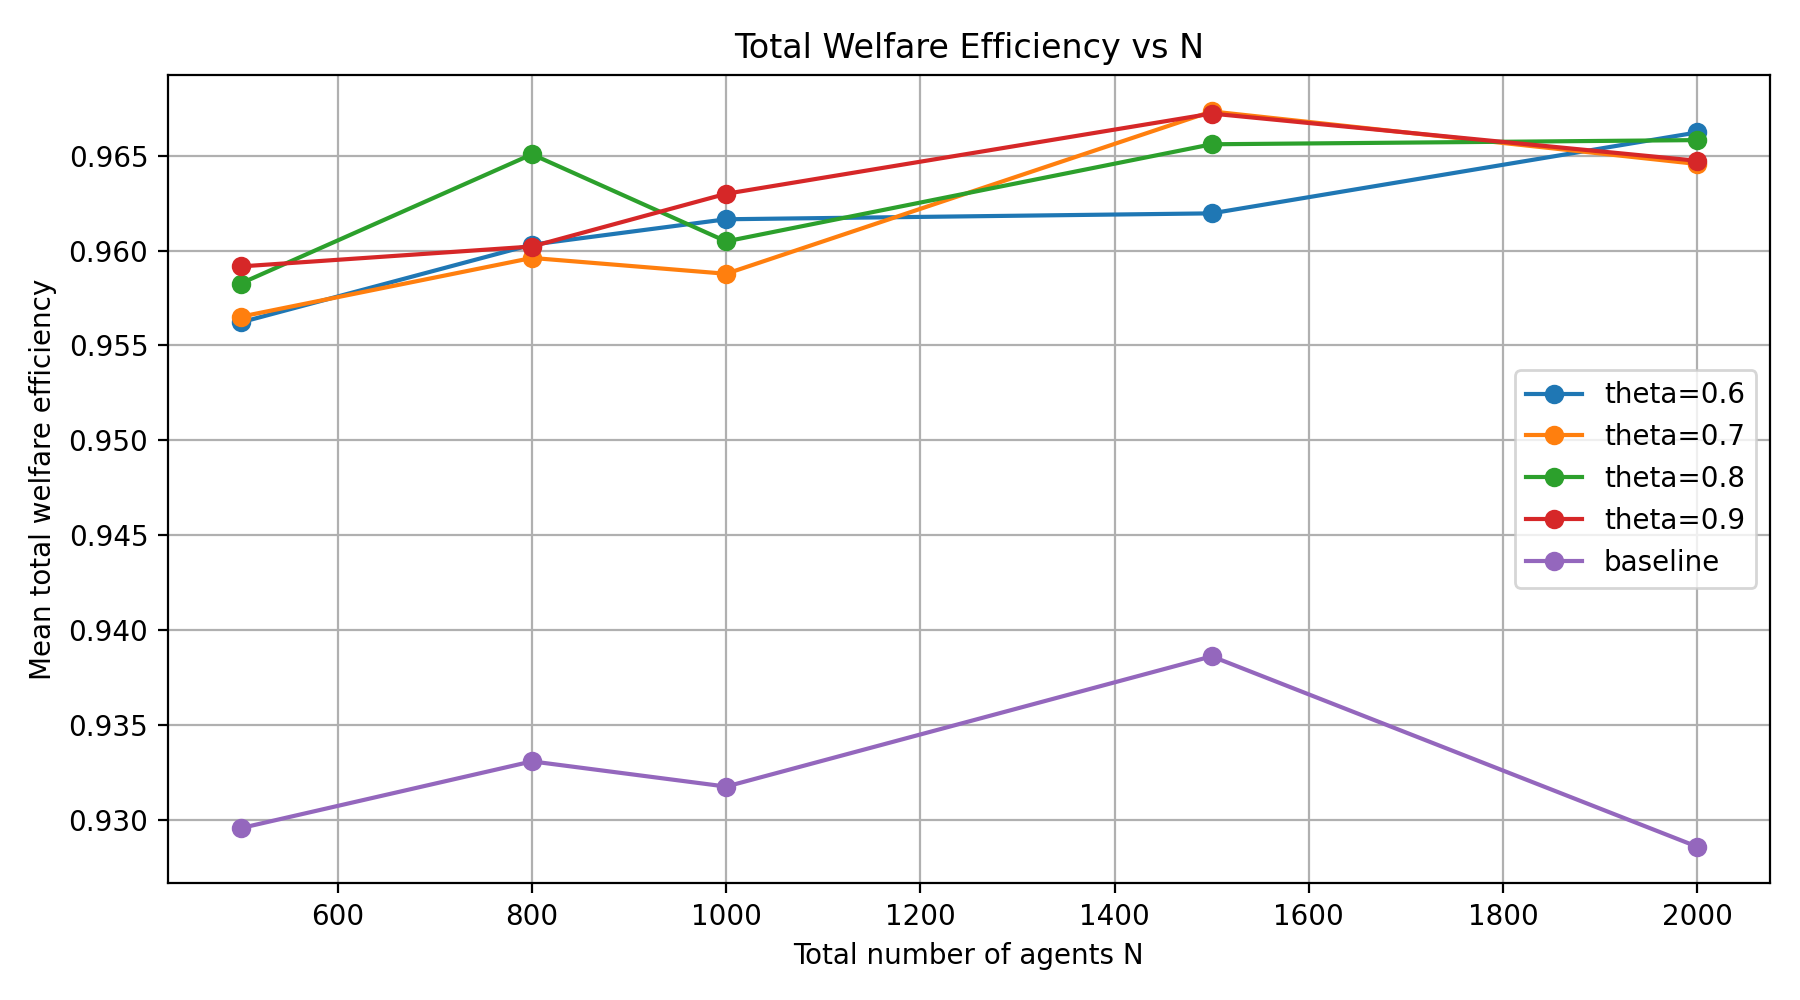
\includegraphics[width=0.92\textwidth]{image/mean_total_efficiency_vs_N.png}
    \caption{不同 balance 阈值下的总社会福利效率}
    \label{fig:mean_total_efficiency}
\end{figure}

图 \ref{fig:mean_total_efficiency} 展示了不同市场规模下的总社会福利效率。可以看到，启用动态 balance 修正后，各组机制的总福利效率均明显高于 baseline。这说明 balance 机制能够缓解分层交易中买卖双方无法充分相遇的问题，使平台在整体资源配置上更接近全局最优。

不过，总社会福利效率整体数值较高，主要是因为 seller 初始持有商品，即使没有交易也会形成基础福利。因此，仅观察总福利效率可能低估分层机制与全局最优之间的真实差距，也可能弱化 balance 修正带来的边际提升。为此，我们进一步观察增量福利效率及其方差。

\begin{figure}[h]
    \centering
    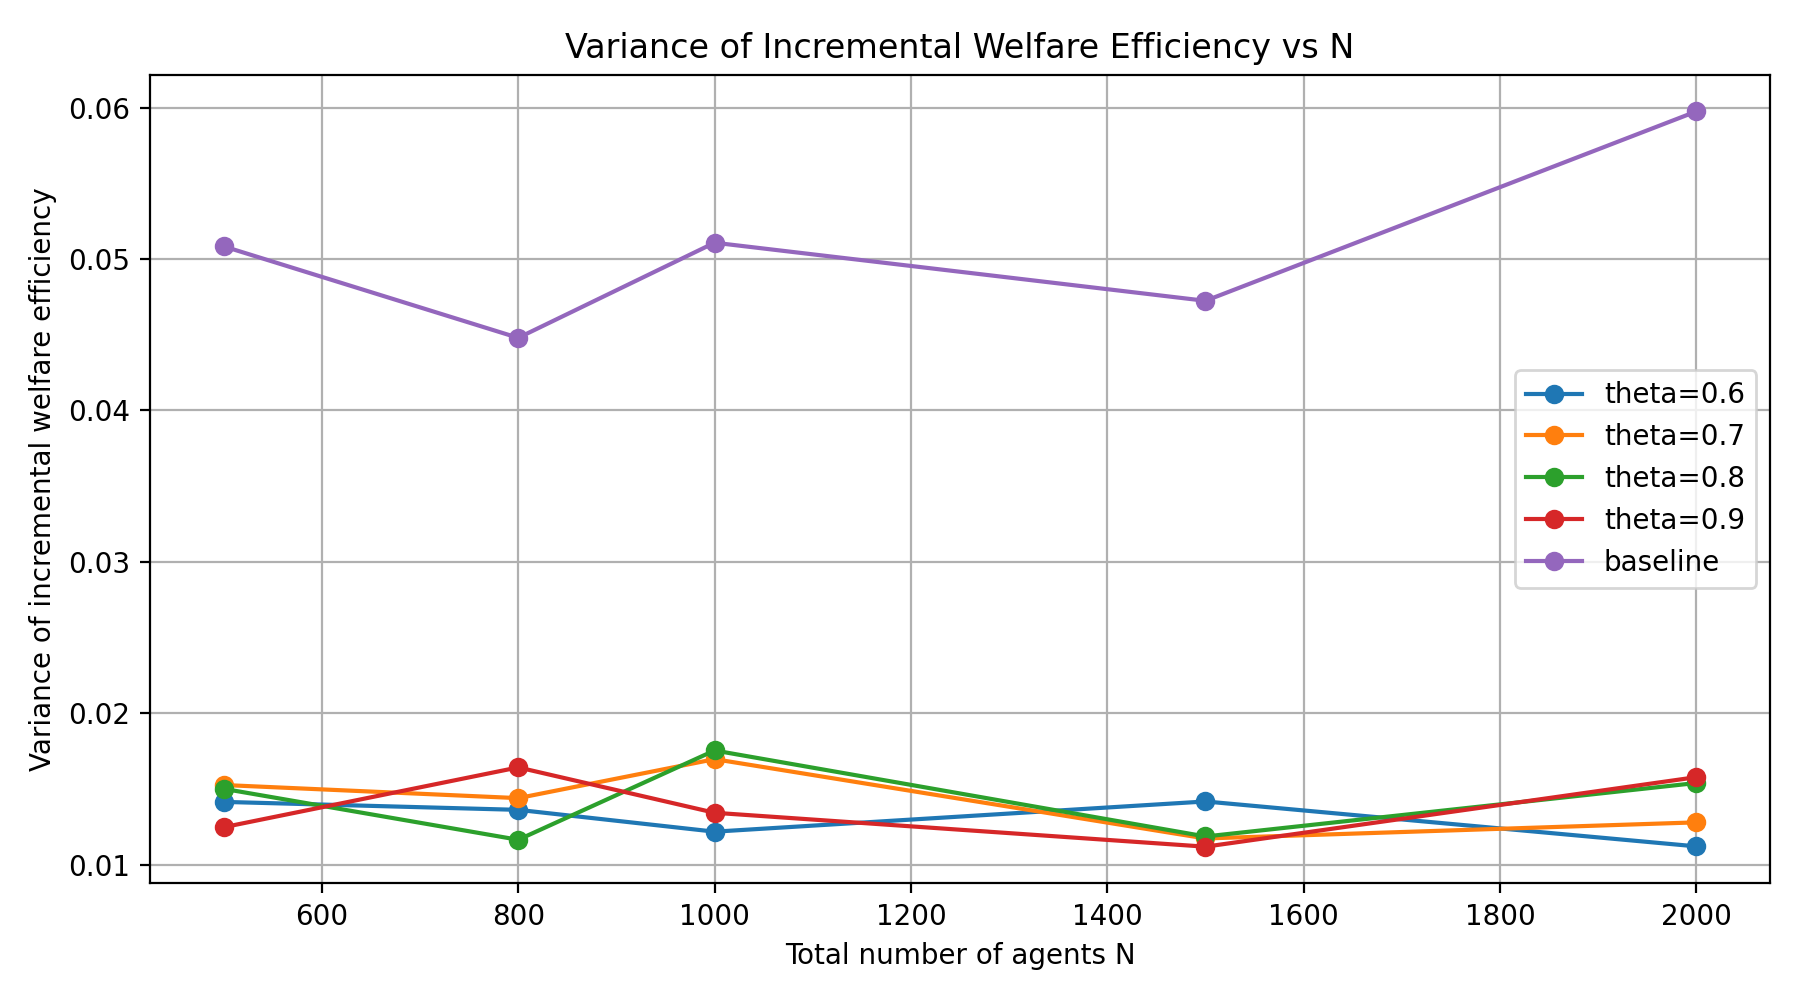
\includegraphics[width=0.92\textwidth]{image/var_surplus_efficiency_vs_N.png}
    \caption{不同 balance 阈值下增量社会福利效率的方差}
    \label{fig:var_surplus_efficiency}
\end{figure}

图 \ref{fig:var_surplus_efficiency} 展示了增量社会福利效率的方差。结果显示，baseline 的方差显著高于启用 balance 修正后的机制。这意味着在不进行 balance 修正时，机制表现更加依赖随机生成的市场结构：若某些层天然买卖双方较为均衡，则机制表现较好；若某些层严重失衡，则成交效率和增量福利会显著下降。

相比之下，动态 balance 机制通过从下一层补充缺失方主体，能够降低不同随机网络之间的表现差异，使机制结果更加稳定。换言之，balance 修正不仅提高了平均效率，也降低了机制对初始网络结构的敏感性。

实验同时表明，balance 阈值并非越高越无条件更优。较高的阈值会促使平台更积极地从下一层市场引入交易主体，通常能够改善当前层流动性并提高平均成交效率；但这种扩展也会提前消耗未来层的潜在交易主体，从而带来一定补充成本。因此，ClearBid 在实际部署中可以根据采购品类和市场成熟度灵活设置 $\theta$：在冷启动阶段适当提高扩展强度以提升流动性；在市场成熟后降低扩展强度以增强稳定性。

总体而言，仿真结果说明：动态 balance 市场扩展机制能够在不改变双边拍卖价格逻辑的前提下，提高局部市场流动性、增加成交机会，并改善供应链采购平台的增量社会福利效率。同时，该机制还能降低平台表现对随机网络结构的依赖，使交易撮合结果更加稳定。
\section{商业模式}

ClearBid 的收入来源包括四类。

\begin{table}[h]
    \centering
    \caption{ClearBid 收入来源}
    \begin{tabularx}{\textwidth}{p{3.2cm}Y}
        \toprule
        收入来源        & 说明                                                           \\
        \midrule
        交易服务费       & 对成功撮合的交易收取小比例服务费，例如按成交额收取 0.5\%--2\% 的平台服务费。早期可采用较低费率吸引用户进入。 \\
        企业 SaaS 订阅费 & 对采购规模较大的企业、园区、学校食堂、连锁餐饮和供应商提供采购管理系统、价格分析报表、供应商管理系统等增值服务。     \\
        数据与风控服务费    & 向金融机构提供脱敏后的企业信用画像、供应链交易报告、价格指数和风险预警服务，按 API 调用、报告数量或年度合作收费。  \\
        供应链金融合作分润   & 当平台向合作金融机构推荐真实交易企业，并促成订单融资、应收账款融资或采购贷时，可在合规前提下获得技术服务费或合作分成。  \\
        \bottomrule
    \end{tabularx}
\end{table}

\section{目标客户与应用场景}

\subsection{第一阶段：生鲜食材采购}

第一阶段聚焦长三角地区中小餐饮企业、学校食堂、社区超市和农产品供应商，选择土豆、蔬菜、猪肉、鸡蛋、大米等高频采购品类作为切入点。

选择该场景的原因是：

\vspace{-0.5em}
\begin{multicols}{2}
    \begin{itemize}
        \item 采购频率高；
        \item 价格波动明显；
        \item 中间环节较多；
        \item 信息不透明问题突出；
        \item 买卖双方数量多；
        \item 真实交易数据具有金融价值。
    \end{itemize}
\end{multicols}

\subsection{第二阶段：低值工业品与办公物资采购}

平台成熟后，可扩展到包装材料、五金件、办公耗材、酒店用品等中小企业高频采购场景。这类商品标准化程度较高，更适合线上双边竞价。

\subsection{第三阶段：医药耗材等强监管场景}

药品和医药耗材采购具有较强监管要求，不建议作为早期主场景。但在平台具备资质审核、合规管理和可追溯交易能力后，可探索与合规医药流通企业合作，进入医药耗材、非处方类商品或机构采购场景。

\section{竞争优势}

\begin{table}[h]
    \centering
    \caption{ClearBid 与其他模式对比}
    \begin{tabularx}{\textwidth}{p{3.5cm}Y}
        \toprule
        对比对象     & ClearBid 的优势                                                        \\
        \midrule
        传统采购平台   & 传统采购平台更多是信息展示和单边报价，ClearBid 强调多买方、多卖方的双边竞价撮合，价格发现能力更强。              \\
        线下批发市场   & 线下批发市场价格不透明、交易记录难沉淀、信用数据难积累。ClearBid 可以形成数字化订单、电子合同、价格指数和信用评分。      \\
        普通电商平台   & 普通电商平台主要服务零售或标准化商品交易，而 ClearBid 面向企业采购，强调批量采购、履约能力、供应链关系和后续金融服务。    \\
        单纯金融风控平台 & 单纯风控平台往往缺少一手交易场景。ClearBid 从真实采购交易切入，天然沉淀订单与履约数据，因此风控数据更真实、更连续、更可验证。 \\
        \bottomrule
    \end{tabularx}
\end{table}

\section{运营与落地计划}

\subsection{冷启动阶段}

平台优先选择一个区域和少数品类进行试点，例如上海及长三角周边的食材采购市场。初期重点引入：

\begin{itemize}
    \item 30--50 家买方企业；
    \item 50--100 家供应商；
    \item 1--2 家物流合作方；
    \item 1--2 家金融机构；
    \item 若干园区或行业协会合作方。
\end{itemize}

平台通过低服务费、免费试用、价格报告赠送、邀请奖励等方式吸引首批用户。

\subsection{试点验证阶段}

重点验证以下指标：

\vspace{-0.5em}
\begin{multicols}{2}
    \begin{itemize}
        \item 买方采购成本是否下降；
        \item 卖方成交机会是否增加；
        \item 平台撮合成功率；
        \item 平均成交周期；
        \item 履约纠纷率；
        \item 用户复购率；
        \item 价格指数是否具有参考价值；
        \item 交易数据是否能够支持金融机构授信判断。
    \end{itemize}
\end{multicols}

\subsection{规模扩张阶段}

当单一区域和单一品类模型跑通后，平台逐步扩展到更多城市和品类，并加强与银行、保理公司、园区、行业协会和大型采购方的合作。

\section{风险与应对措施}

\begin{table}[h]
    \centering
    \caption{主要风险与应对措施}
    \begin{tabularx}{\textwidth}{p{3.5cm}Y}
        \toprule
        风险类型            & 应对措施                                                                                                \\
        \midrule
        商品质量不一致风险       & 建立标准化商品分类、质量等级、验收标准和评价体系，对不同等级商品分别形成价格指数，避免低质低价扰乱市场。                                                \\
        商品异质性导致双边拍卖失真风险 & 对大类商品设置标签向量，将品类、规格、质量等级、产地、交付区域、交付时间窗和验收标准相同或可替代的商品放入同一交易池；标签差异较大的商品分池竞价，避免不同质量商品被错误比较。             \\
        虚假报价与恶意竞价风险     & 引入保证金机制、报价信用分、异常报价识别和违约惩罚机制。多次虚假报价的用户将被降低信用等级或限制交易。                                                 \\
        邀请激励被滥用风险       & 只对补充前已锁定、真实成交且履约完成的邀请关系给予奖励；balance 补充产生的新增交易不直接进入原邀请奖励池，并通过图谱异常检测识别循环邀请、密集关联账户和异常交易集群。             \\
        Sybil 小号与互刷风险   & 将用户最终可信度拆分为行为可信度与 Sybil 风险；对星型小号树、长链邀请、兄弟节点高度相似、同父互评团和低外连高内聚社群进行识别，并对群内评价降权、同源奖励封顶、必要时触发身份复核。       \\
        身份信息重复计分风险      & 身份验证只作为降低 Sybil 风险的修正项，不直接进入行为可信度；地址、银行卡、收款账号等信息只有在必要、可验证且合理唯一时提高验证等级，若出现共享、冲突或频繁变化，则计入信息异常或设备异常风险。 \\
        价格公开带来的隐私风险     & 只发布脱敏后的聚合价格指数，不公开单个企业的采购价格、交易对象和合同细节。                                                               \\
        金融合规风险          & 平台定位为技术服务和交易数据服务平台，不直接发放贷款。金融服务由持牌银行、保理公司和小贷机构提供。                                                   \\
        \bottomrule
    \end{tabularx}
\end{table}

\section{发展愿景}

ClearBid 的长期目标是成为面向中小企业采购场景的透明交易基础设施。平台通过双边拍卖机制提升价格发现效率，通过邀请机制扩大市场流动性，通过真实成交数据形成可信价格指数和企业信用画像，最终构建“采购交易—价格透明—履约信用—供应链金融”的闭环。

未来，ClearBid 可从生鲜食材采购扩展到工业品采购、办公物资采购、酒店用品采购、医药耗材采购等多个场景，并与金融机构、园区、行业协会和政府部门合作，为中小企业提供更加透明、高效、可信的数字化采购与金融服务。

\section{项目一句话总结}

ClearBid 透明采购不是普通电商平台，而是一个基于双边拍卖机制的供应链采购价格发现与金融科技平台。它通过聚合买卖双方报价，让真实成交价格更加透明；通过邀请激励机制扩大市场规模；通过履约数据和交易记录形成信用画像，为中小企业采购降本和供应链金融风控提供基础设施。

\end{document}